% Figures -- architecture + 3 result charts. Put the PNGs next to main.tex
% (or set \graphicspath{{paper_figures/}}).
\begin{figure}[t]\centering
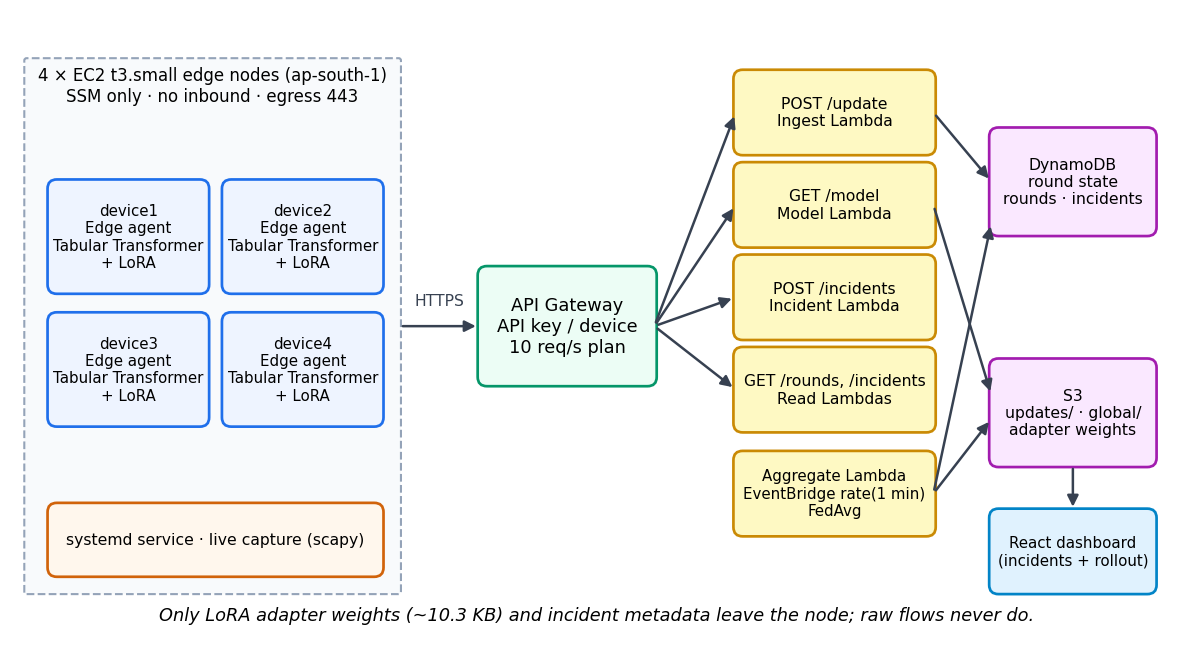
\includegraphics[width=\columnwidth]{fig1_infrastructure.png}
\caption{Agentic FedGrid architecture: four EC2 edge agents (perceive--decide--act--reflect) exchange only LoRA adapters and incident metadata with a serverless AWS control plane (API Gateway, Lambda, DynamoDB, S3).}
\label{fig:arch}
\end{figure}

\begin{figure}[t]\centering
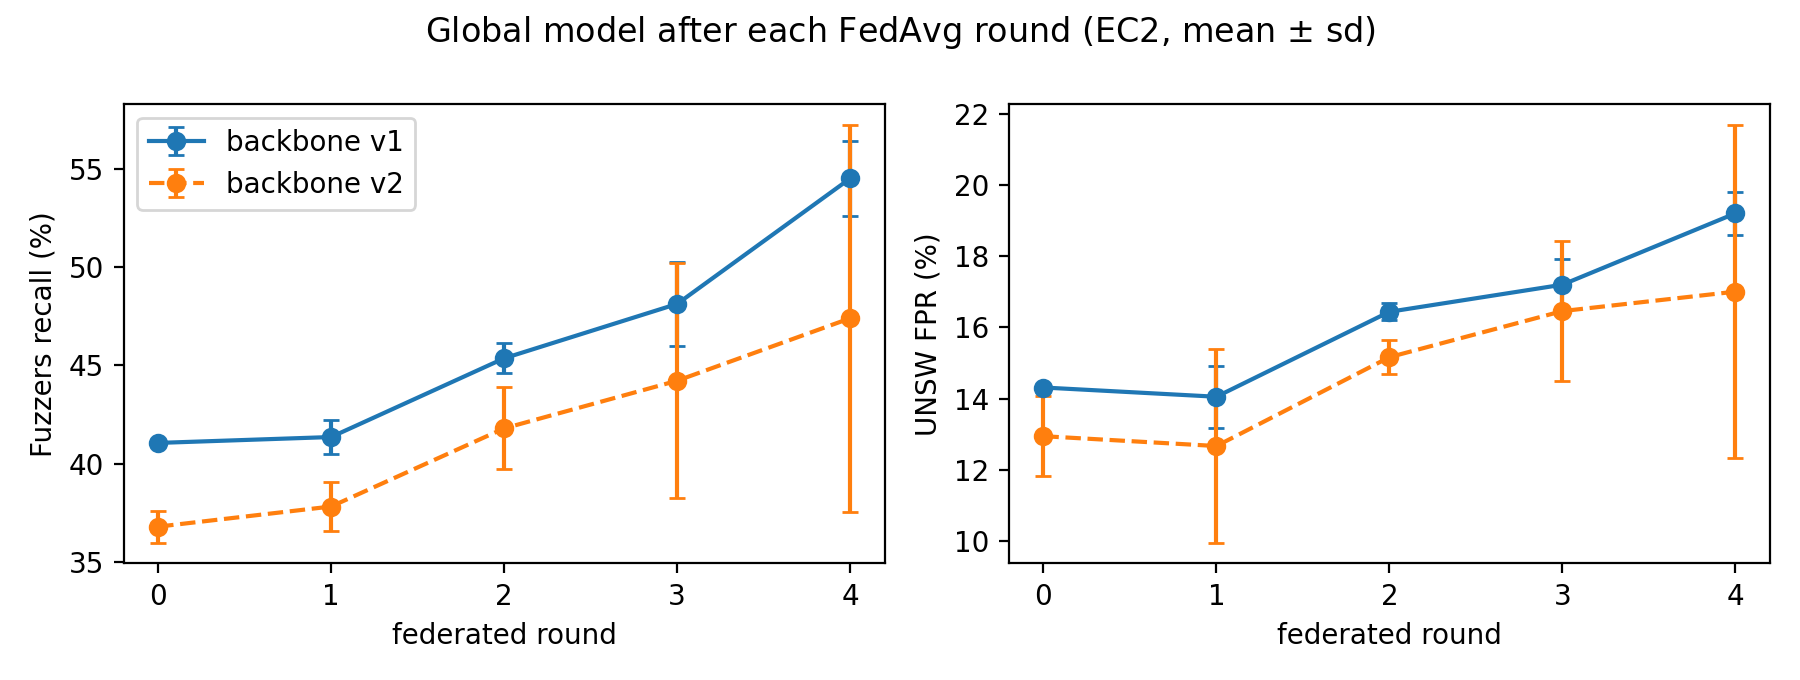
\includegraphics[width=\columnwidth]{fig2_rounds.png}
\caption{Global model per FedAvg round on device~2 (never sees Fuzzers locally): Fuzzers recall at the default threshold (left) and UNSW-NB15 FPR (right), mean $\pm$ sd over seeds, EC2. Both rise together; moving the frozen backbone's threshold to the same FPR gives the same recall (Table~\ref{tab:threshold}).}
\label{fig:rounds}
\end{figure}

\begin{figure*}[t]\centering
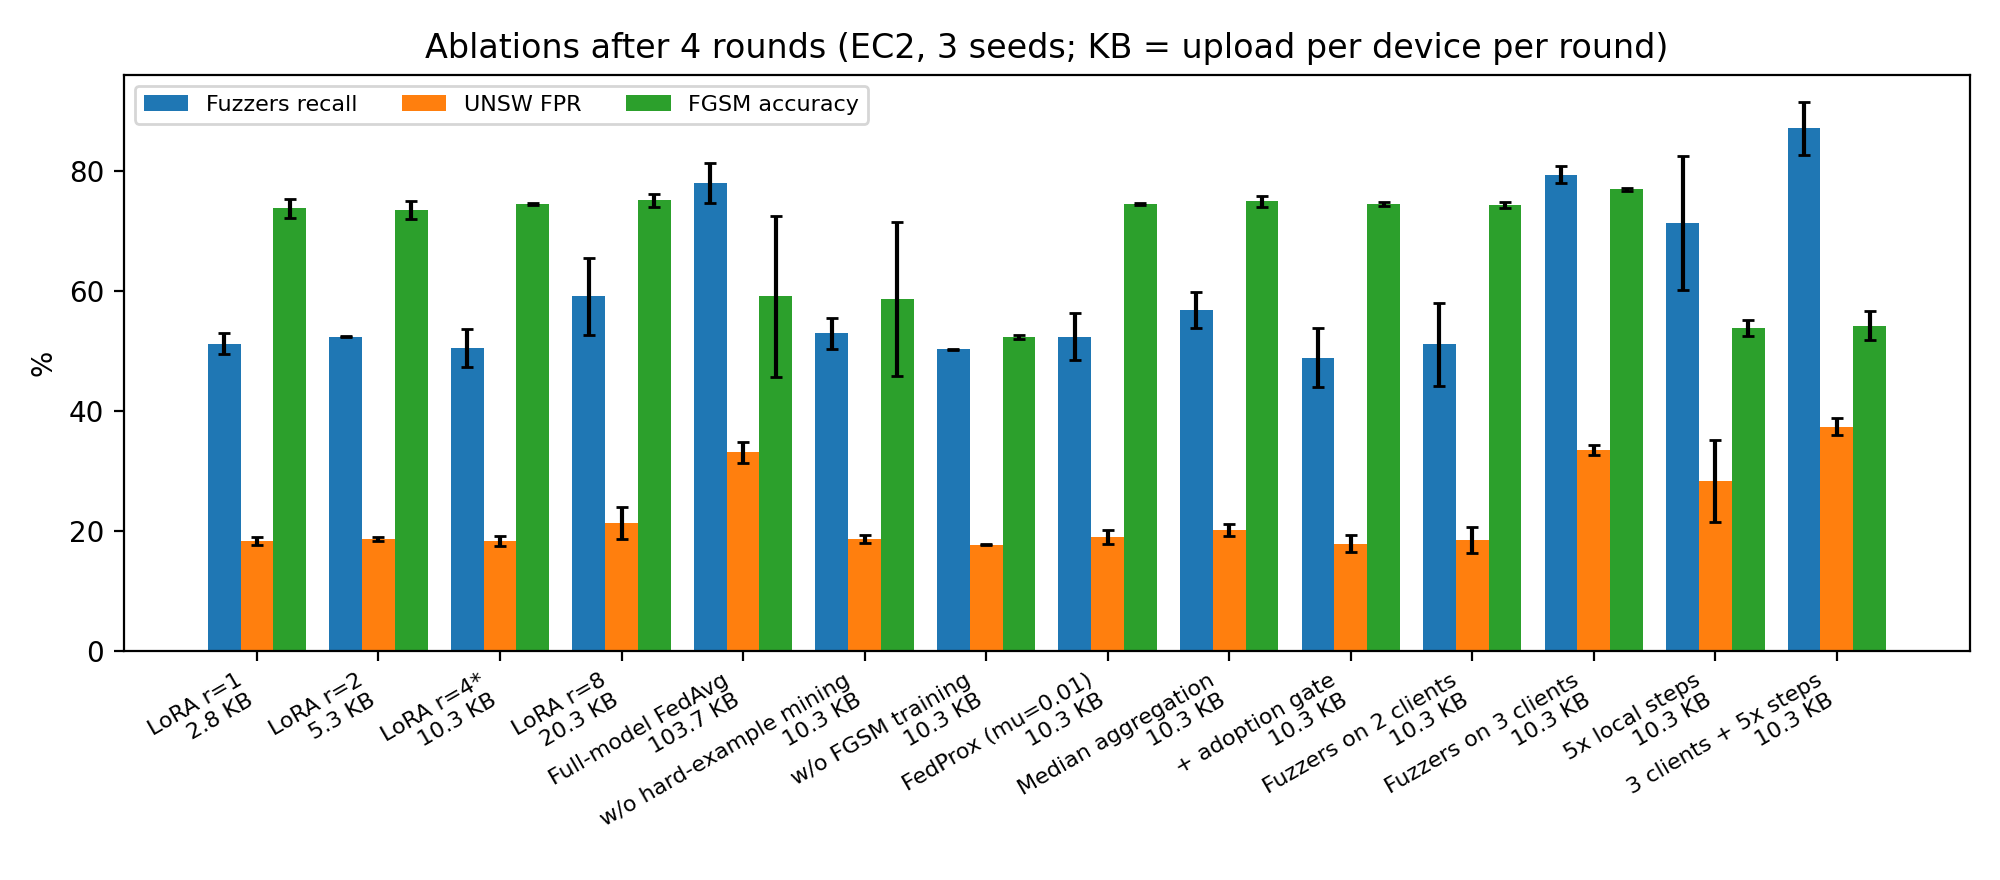
\includegraphics[width=0.9\textwidth]{fig3_ablation_bars.png}
\caption{Ablations after four rounds (3 seeds, EC2). Labels give the upload size per device per round. Poisoning results are in Table~\ref{tab:ablation}.}
\label{fig:ablation}
\end{figure*}

\begin{figure*}[t]\centering
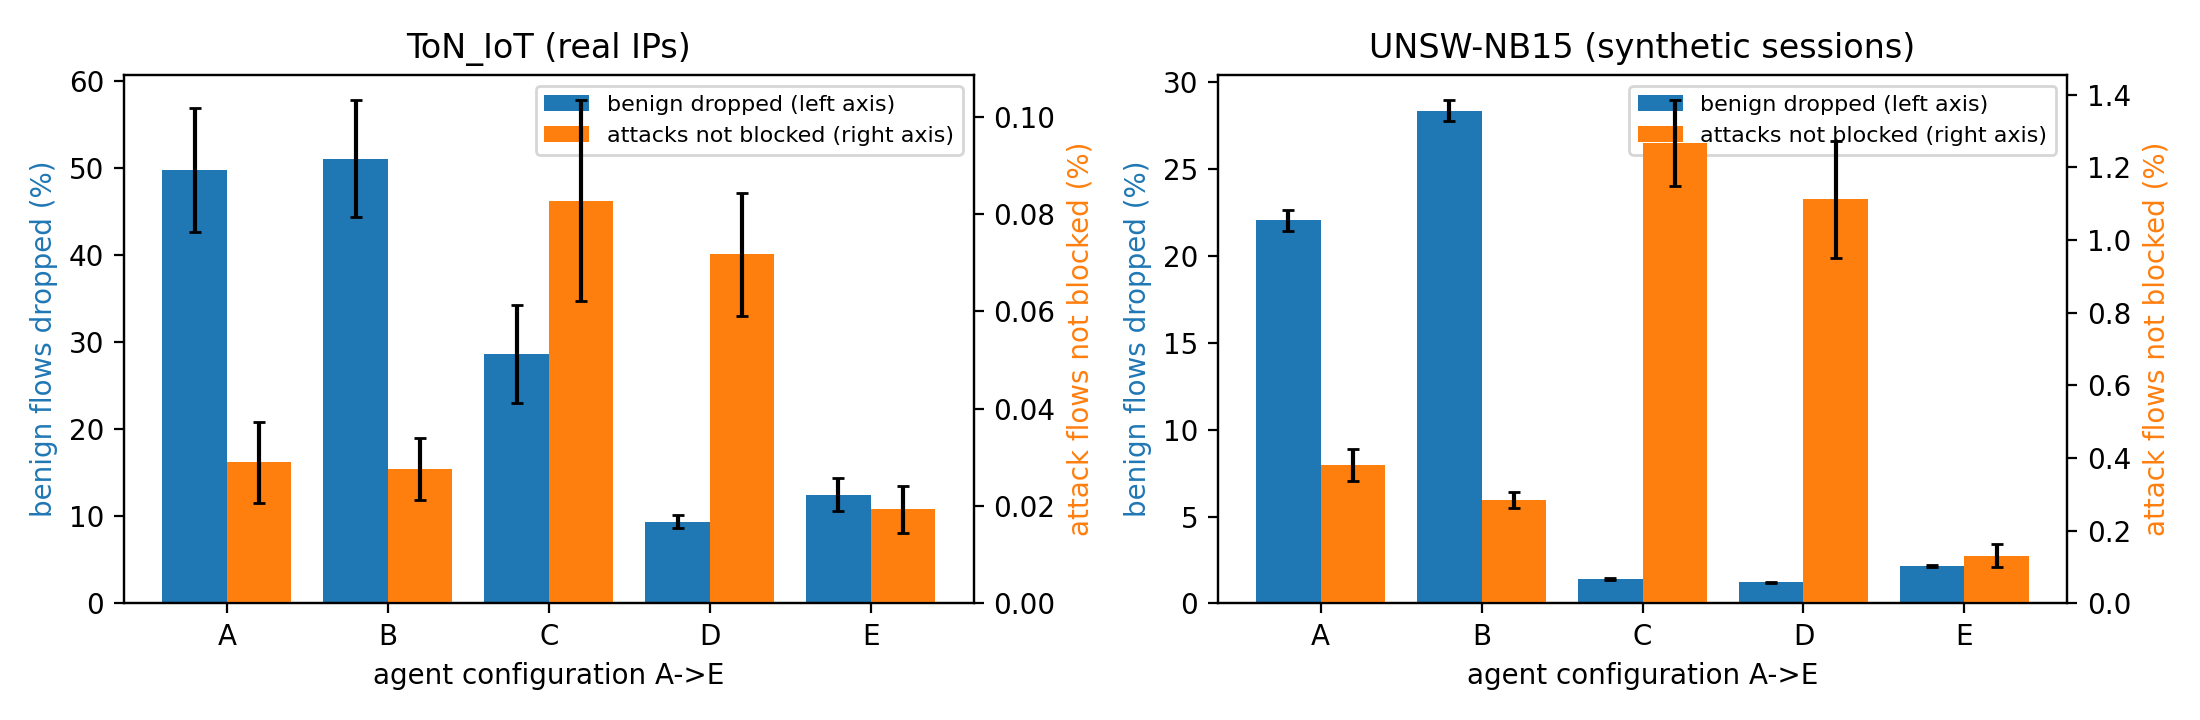
\includegraphics[width=0.9\textwidth]{fig4_agent_bars.png}
\caption{Agent configurations A (threshold, permanent block) to E (full agent): benign flows dropped and attack flows not blocked, four agents, 3 seeds.}
\label{fig:agent}
\end{figure*}
